\documentclass[conference]{IEEEtran}


  	\usepackage[pdftex]{graphicx}
  	\graphicspath{{../pdf/}{../jpeg/}}
	\DeclareGraphicsExtensions{.pdf,.jpeg,.png}

	\usepackage[cmex10]{amsmath}
	\usepackage{mathabx}
	\usepackage{algorithmic}
	\usepackage{array}
	\usepackage{mdwmath}
	\usepackage{mdwtab}
	\usepackage{eqparbox}
	\usepackage{url}
	\hyphenation{op-tical net-works semi-conduc-tor}
\usepackage{hyperref}
\hypersetup{
    colorlinks=true,
    linkcolor=blue,
    filecolor=magenta,      
    urlcolor=cyan,
    pdftitle={Overleaf Example},
    pdfpagemode=FullScreen,
    }

\urlstyle{same}

\begin{document}

\title{\LARGE Online Hotel Booking Recommendation System}

% \author{\authorblockN{Leave Author List blank for your IMS2013 Summary (initial) submission.\\ IMS2013 will be rigorously enforcing the new double-blind reviewing requirements.}
% \authorblockA{\authorrefmark{1}Leave Affiliation List blank for your Summary (initial) submission}}

 \author{\authorblockN{Nikhil Dutt (A14285637) \authorrefmark{2}, Abhishek Khare (A59010306) \authorrefmark{2} }
}

\maketitle

\begin{abstract}
Planning a vacation or weekend escape can be an overwhelming affair because with thousands of hotels to choose from it’s difficult to know which one would suit your personal preferences. So in order to simplify this process we plan to create a recommendation strategy for hotel booking. We would use data analysis techniques for pre-processing/standardizing the data, and make inferences based on the statistical analysis of the data. We would use various statistical classification strategies and then perform hypothesis testing and then make conclusions based on it.
\\
\\ Project Type: Data exploration and inference.
\\
\end{abstract}

\IEEEoverridecommandlockouts
\begin{keywords}
Logistic Regression, Bayesian Decision Rule, Support Vector Machines (SVM), Decision Tree
\end{keywords}

\IEEEpeerreviewmaketitle


% ===================
% # I. Introduction #
% ===================

\section{\textbf{Introduction}}
The Expedia Group wants to eliminate any inconveniences and difficulties from their hotel search process by providing personalized hotel recommendations to their users. Given that this site sees hundreds of millions of visitors every month, this task involves a lot of complexities.
\subsection{Problem Statement:}
Designing a fairly reliable and accurate recommendation system for online hotel booking based on data analysis and statistical machine-learning techniques applied to the existing dataset. 
\subsection{Problem Description:}
Currently, Expedia makes use of search parameters to adjust their hotel recommendations, but there isn't enough customer-specific data to personalize them for each user. In this task, we aim to contextualize the customer data and predict which hotel group (out of 100 different hotel groups) a user will be most likely to stay at. To do this, we will use different techniques including Logistic Regression, Bayesian Decision Rule, Support Vector Machines, Decision Trees and compare the results of each to determine the most successful approach. Along with this, we will identify the key drivers or features that lead to successful recommendations.
\subsection{Project's Significance:}
This problem is significant as every company aims to maximize its profitability and to do that they must ensure that they retain customers by providing them with high-quality services. Insights from customer-specific data as well as a recommendation system can allow the business to generate more accurate recommendations and attract more users.  
\subsection{Target Questions and Inferences:}
Our goal is to find answers to questions like - What are the user preferences when booking a hotel? Do users books a hotel as a part of a package deal? Do mobile users make a booking more frequently than other users? Which month/season gets more online bookings? What is the statistical distribution of the users' duration of stay? etc. 
% =======================================================
% # II. Impact of traps on large signal characteristics #
% =======================================================

\section{\textbf{Description of Dataset}}
For this project, we have used a publicly available dataset from Kaggle which includes logs of Expedia's customer behaviour. This data is separated into two different sets: the test data (used only for evaluating performance of our models) and the training set (which will be used for data exploration and training our models). These two sets are split based on time: training data are from 2013 and 2014, while test data are from 2015. Upon further inspection of the data we see that we are provided with 24 different features. Our target variable (the one we are trying to predict) is ‘hotel-cluster’ and we will essentially use the other 23 variables (depending on which ones we deem useful) to make a prediction for a hotel cluster. These hotel clusters serve as good identifiers to which types of hotels people are going to book, while avoiding outliers such as new hotels that don't have historical data. 


% =============================================
% # III. Modeling and consistency validations #
% =============================================

\section{\textbf{Data Exploration}}

In our training data, we have 200,000 rows (customer logs) and 24 columns. After performing some basic data cleaning, we find that three features have missing data: distance from origin to destination, check-in date and check-out date. Since check-in and check-out date account for less than 1\% of the missing data, it would make more sense to drop these records since it would be extremely difficult to impute these. Distance from origin to destination accounts for 34\% of the missing data so we must implement a data imputation strategy for these records. We simply replace missing values in this field with the mean distance from origin to destination of the entire training set. After these changes, we are now working with a training set that has 199,823 instances.

\textbf{Correlation Analysis:} For this type of analysis we will be using the concept of correlation from class. We will be using the Pearson coefficient to determine the degree to which each feature is correlated with each other. When the coefficient is closer to +1, 0, and -1, we have that the pair of features is strongly positively correlated, uncorrelated and strongly anti-correlated respectively. The following formula was used to calculate the Pearson coefficient:
\begin{figure}[ht!] %!t
\centering
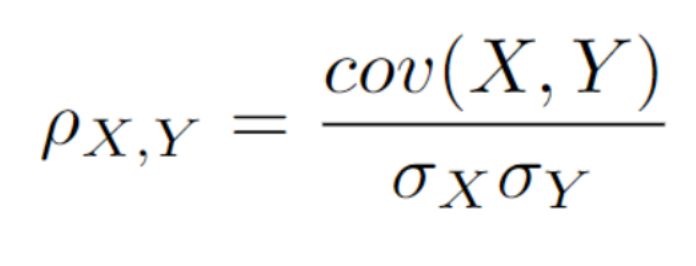
\includegraphics[width=1.5in]{pearson.PNG}
\label{pearson}
\end{figure}

Figure 1 shows a heatmap containing the correlation coefficients between various features of the training set. Darker colors denote low correlation and brighter colors denote higher correlation. Nothing interesting really stands out here as most features do not seem to be correlated with hotel cluster and the features don't seem to be correlated among themselves. Ideally if we saw that certain features were highly correlated with each other, we would remove one of them since we would not want the effect of that particular variable to appear twice in the model. Since we see that none of the attributes correlate very well with each other, we can proceed by using all the attributes in the dataset.

\begin{figure}[ht!] %!t
\centering
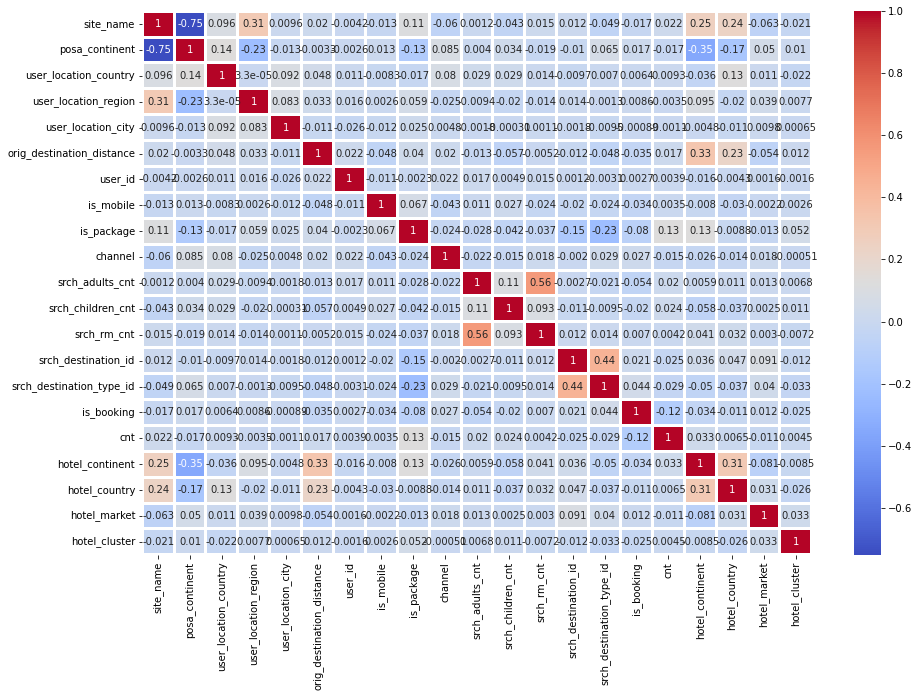
\includegraphics[width=3.5in]{heatmap.png}
\caption{Correlation among all features in the dataset}
\label{heatmap}
\end{figure}
While conducting basic exploratory data analysis, we observed that overall the number of bookings through mobile phones is less compared to bookings through the Expedia website as seen in Figure 2. This information could be used to suggest that Expedia make a more interactive and easy to use website so that users can book their hotels with greater ease. Additionally, we see that most bookings made were not part of a travel package (less than half of the bookings were through a package).

There are 6 different continents in this dataset as seen in the figure. 'posa\_continent' refers to the continent from where a specific booking was made while hotel\_continent refers to the continent where the booking was for. We can see that majority of bookings are made from the site in Continent 3. There could be a variety of reasons for this such as people there having more expending power. Expedia could possibly increase its business by increasing more hotel options, more variety, better user experience, etc. For other continents Expedia can lower its prices on hotels and provide discounts or loyalty points. The figure also tells us that while most bookings are made from Continent 3, the majority of the booking destinations are in Continent 2. That is, most people are from Continent 3 and travel to Continent 2. In figure X we see data for each month across three years and that the highest number of bookings was consistently in the month of August. It is likely the case that most users book in this period as it is the peak of the summer holidays.

In our analysis it was clear that 2014 had the most number of bookings. If we take a look at figure X which shows month wise bookings, the graph peaks at certain months in 2014 and clearly exceeds bookings made in 2013. We then see that the number of bookings in 2015 decreases heavily. Therefore, it might be a good idea for Expedia to compare what was the strategy in 2014 versus 2015 which caused such a considerable decline in the number of bookings.



\begin{figure}[ht!] %!t
\centering
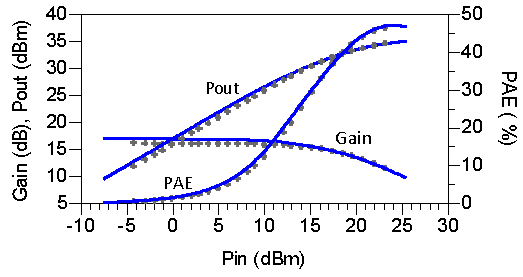
\includegraphics[width=3in]{FigureLP_ancien_mod.pdf}
\caption{Measurements (grey), modeling (blue) of the CW RF performances of a 8x75$\mu$m AlInN/GaN HEMT at 10.24GHz in class AB. $Z_{loadOPT} = (20+j.18) \Omega$.}
\label{LP}
\end{figure}

However, using this model, the transient dynamics of the average current during pulsed power RF measurements is not sufficient as was already observed in \cite{9257290}.
Even if the output current behavior, due to capture and release of charges by traps is consistent as both processes are taken into account, the amplitude of the discontinuity of the current (named $\Delta I_{D1}$ in Figure \ref{Courant_2}), observed at the moment when the RF signal is switched off, has not enough amplitude. This can be explained by the fact that the extraction of the drain-lag contribution from pulsed-IV measurements at different quiescent bias points is a too much rough method to provide a correct traps induced current dispersion, especially around the nominal bias point, which is moreover often at low current in amplifiers. This however allows to model enough precisely the IV characteristics in the area of the IV network where the current is high and the drain voltage is close to the knee voltage, and where the traps induced current dispersion limits the RF load lines swing under RF power drive. This explains the good capability of the previous model to fit RF power characteristics despite the use of pulsed IV networks to model the lag correction terms.

We propose here to use low-frequency S-parameters measurements instead or in addition to pulsed IV measurements, which represent a far more precise and convenient method to extract the drain-lag contribution in the transistors non-linear models. Precise because the S-parameters do not provide the current, but directly its derivative. The output conductance is expressed by $g_d=\Re \left\{Y(2,2)\right\}$. $g_d$ is very sensitive to the drain-lag trapping effects, in the frequency range of the emission time constants of these traps.

Convenient because the variations of the output conductance also provide the detrapping and thermal time constants, and give the ability to separate both effects, which induce opposite $g_d$ variations. However, traps time constants are particularly dependent on the electric fields and the temperature conditions (i.e. the measurement bias point), and these variations are not taken into account in the drain-lag model for the moment. Thus, the modeled traps time constants are fixed at the values measured with low frequency S-parameters at the nominal bias point of the application.

The amplitude of the correction term is also determined from the same measurement, at the nominal bias point, in order to get the correct dispersion level in pulsed RF case, when RF is switched off and the transistor goes back to its nominal bias point. This however highlighted an imprecision of the previous model, in which the dispersion correction term was added to the command voltage vgs. Indeed, the fit of the output conductance dispersion induced by trapping effects leaded to a too high level of dispersion at high current, i.e. where the RF signal swings during power RF operation, thus inducing too much power slump in such cases. The model has been modified in order to add this correction term to the pinch-off voltage ($v_p$) formulation and also to the parameter $I_{DSS}$ (determining the steady state current) into the current source equations. Both contributions are written in order to conserve the proportionality relationship between $v_p$ and $I_{DSS}$. It allows to get a more precise dependence of the dispersion versus the current Ids delivered by the current source.

\begin{figure}[ht!] %!t
\centering
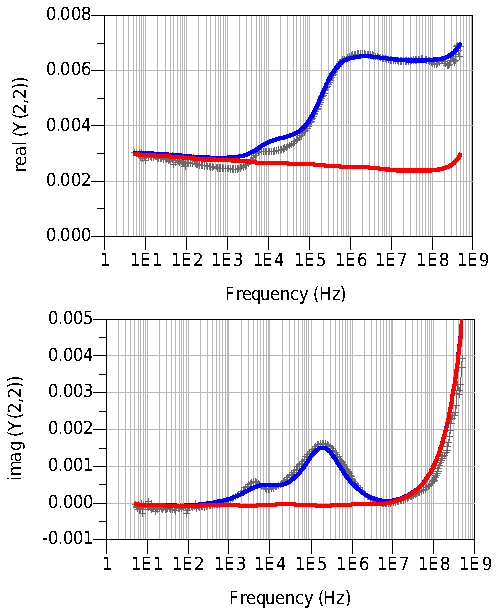
\includegraphics[width=3.0in]{Compare_S.pdf}
\caption{$\Re\{Y_{22}\}$ and $\Im\{Y_{22}\}$. AlInN/GaN 8x75 $\mu m$ HEMT measurements at $V_{ds}=20V$, $I_{ds}=120mA$ (grey) are compared to a simple eletro-thermal model (red) and an eleectro-thermal model including activated drain-lag effects (blue)}
\label{Compare_S}
\end{figure}

A low-frequency S-parameters comparison between measurements and simulation at $V_{ds}$=20V, $I_{ds}$=200mA/mm is presented at Figure \ref{Compare_S}. The measurements have been performed between 5Hz and 500MHz in order to capture all the variations range of the thermal and trapping effects.

We can observe two main traps having emission time constants leading to an increase of gd in the range of 2kHz-8kHz and 20kHz-1MHz, respectively. Thermal effects induce a decrease of the output conductance. The thermal model was determined from a three-dimensional finite element (3D-FE) simulation, and in order to take into account the distribution of the time constants, five RC-cells (i.e. five time constants) are necessary. However, the thermal contribution on the output conductance is quite negligible, as can be seen on the red curve that corresponds to the model with thermal effects only (trapping effects are desactivated).

The imaginary part of $Y(2,2)$ is also presented, and a good agreement between the measurements and the simulations with this non-linear electrothermal model can also be observed. One can see that this imaginary part exhibits two maxima, which correspond to two kinds of drain-lag inducing traps. Thus this kind of measurement provides a convenient way to identify various types of traps in the transistor. 

\begin{figure}[ht!] %!t
\centering
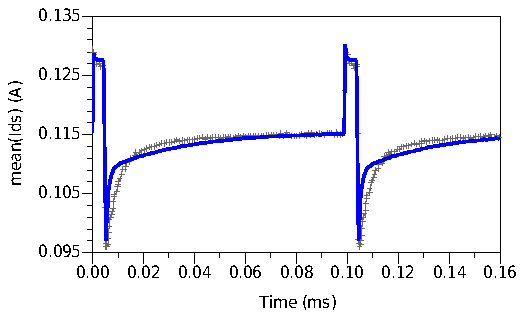
\includegraphics[width=3.0in]{Compare_pulse.pdf}
\caption{Measurements (grey) and modeling (blue) of the average output current in pulsed RF signal operation at 10 GHz (5$\mu$s-100$\mu$s) with DC bias (20V, 115 mA). The amplitude of the transcient induced by detrapping when RF is switched off is accurately modeled.}
\label{Compare_pulse}
\end{figure}

Figure \ref{Compare_pulse} shows a comparison between RF pulsed measurements and simulations with this model. The transistor is measured at Vds0=20V, Ids0=115mA (190mA/mm), on a load impedance $Z_{load}=\left(20+j18\right)\Omega$. The bias voltages are continuous, and the RF signal, at a frequency of 10GHz, is pulsed. Its duration is 5$\mu s$, and its period 100$\mu s$. On this example, the RF imput power equals 20dBm, corresponding approximately to 1dB of gain compression. The very large amplitude of the current discontinuity at the moment when RF is switched off leads to a transient current from 97mA to 115mA (i.e. the nominal bias point). 

Envelope-transient simulations show the modeled output current, and the model enhanced capability to reproduce both the current discontinuity and the slow transient due to traps emission. The emission time constants are however not very accurate, and this can be due by the strong non-linearity of traps time constants versus bias and temperature, as explained previously.


% ==================
% # IV. CONCLUSION #
% ==================

\section{\textbf{Binary and Multi-Class Classification Techniques:}}
For the classification problem, we need to basically make two types of classifications and answer/predict the following two unknowns.
\begin{itemize}
\item Whether the given user would make a booking ? - This involves Binary Classification as we have a yes/no answer.
\item User hotel cluster preference - This involves Multi-Class classification as we need to predict which cluster of the hotels would the user prefer. The given Expedia dataset contains 100 hotel clusters and the classifier has to predict which of those hotel cluster has the better chances of getting picked by the user and would thus be recommended to the user.
\end{itemize}

\subsection{Classification Methods:}

\subsubsection{Naive Bayes Decision Classifier:}
To be filled.

\subsubsection{Support Vector Machines}
To be filled.

\subsubsection{Decision Tree}
To be filled.

\section{\textbf{Hotel Cluster Classification:}}
In order to classify which cluster of hotels would be the user's choice we would use various machine learning methods and would train these ML classifiers on the dataset. For this project, we have tried classification methods like - Support Vector Machines, Naive Bayes Decision Classifier, and Decision Tree Classifier. \\
We standardized the input training vector data and then applied these methods and set the hyperparameters based on the standard hyperparametric optimization techniques.\cite{9257290}

\begin{table}[htbp]
\begin{tabular}{|c|c|}
\hline
\textbf{Classification Technique} & \textbf{Cluster Classification Accuracy} \\ \hline
SVM (Linear Kernel)               & 52.4 \%                                  \\ \hline
SVM (RBF Kernel)                  & 61.2 \%                                  \\ \hline
Naive Bayes Decision Rule         & 59.2 \%                                  \\ \hline
Decision Tree                     & 68.5 \%                                    \\ \hline
\end{tabular}
\end{table}
\section{\textbf{User Decision Prediction}}
Whether a user makes a booking or not.
To be Filled
\section{\textbf{Predictive Task}}
\textbf{Logistic Regression (LR)}: Logistic Regression is similar to linear regression except that logistic regression predicts if something is true or false rather than predicting something continuous. Additionally instead of fitting a line to the data, logistic regression fits an ‘S-shaped’ logistic function and hence is primarily used for classification. LR models the chance of an outcome based on individual characteristics. Since chance is a ratio what actually gets modeled is the logarithm of chance given by:
\begin{figure}[ht!] %!t
\centering
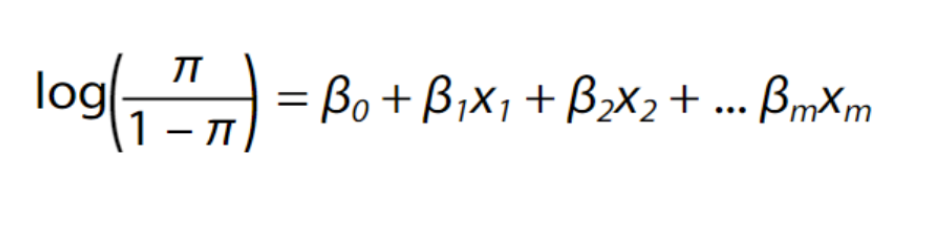
\includegraphics[width=3in]{LR.PNG}
\label{pearson}
\end{figure}

where $\pi$ is probability of an event (e.g. belonging to a hotel cluster in our case), \(\beta_i\) are the regression coefficients and \(x_i\) are the predictive variables or features. 



% ==================
% # ACKNOLEDGMENTS #
% ==================

% use section* for acknowledgement
%\section*{Acknowledgment}
% The authors would like to thank...


% ==============
% # REFERENCES #
% ==============

\section{\textbf{Results and Conclusions}}
To be Filled.
\section{\textbf{Inferences}}
We can make the following inferences based on our exploration.
\begin{itemize}
  \item Mobile Users - The majority of the users who intend to search for hotels or make a booking are not doing so on a mobile device.
  \item Seasonal Preferences - On a Global scale, we observed that hotel bookings are affected by seasonal differences, and the months of August to December see a higher number of hotel bookings when the northern hemisphere experiences Fall and winter. (Majority of the world population lives in the northern hemisphere)
  \item Regional Preferences - We have observed that the majority of the bookings are done from Continent id - 2 and are made for booking hotels in continent id - 3. (continent names redacted for user data privacy).
  \item Package Deals - Majority of the users booked the hotels which were not a part of a package deal offered by the agency.
\end{itemize}

\section{\textbf{Project Member Contribution}}
\begin{table}[htbp]
\begin{tabular}{|c|c|c|}
\hline
Member Name    & Hours Contributed & Contribution Percentage \\ \hline
Nikhil Dutt    & 25                & 50 \%                   \\ \hline
Abhishek Khare & 25                & 50 \%                   \\ \hline
\end{tabular}
\end{table}

\section{\textbf{Resources}}
\noindent Project Repository - \href{https://github.com/abhishekkhare1998/Hotel-Booking-Recommendation}{Github Link}.\\
 Dataset Used - \href{https://www.kaggle.com/competitions/expedia-hotel-recommendations/data}{Kaggle Link}
\bibliographystyle{IEEEtran}
\bibliography{IEEEabrv,biblio_traps_dynamics}

\end{document}
